


\section{Case Study}\label{sec:sim}
In this section, we introduce the use case employed to generate our results. We used the Stonefish simulator \cite{cieslak2019stonefish, grimaldi2025stonefishsupportingmachinelearning} to model a multi-agent AUV mission operating under shared autonomy in a submerged environment. In such complex settings, AUVs benefit greatly from human oversight, especially when perception and decision-making are affected by uncertainty. By incorporating a Human-in-the-Loop (HITL) approach, operators are able to intervene in critical processes such as perception, communication, and knowledge enrichment, thereby enhancing mission reliability and adaptability. Both the human operator and the robot can dynamically update the knowledge graph and the taxonomy.

Figure \ref{fig:use_case_system_architecture} illustrates the autonomy framework, emphasizing the interaction patterns and decision-making flow that characterize shared autonomy. The scenario features two AUVs, each with distinct capabilities and roles:
\begin{itemize}
\item \emph{Alpha} is equipped with RGB and depth cameras and serves primarily as the survey unit.
\item \emph{Beta} is equipped with RGB and depth cameras as well as an underwater manipulator, making it primarily responsible for intervention tasks.
\end{itemize}

\noindent Both robots are also equipped with a VLC sensor that allows them to exchange information with each other. Additionally, the robots also have access to a docking station through which they can use the VLC sensor to communicate with the human operator.  

In this case study, the AUVs are deployed to explore a marine environment in search of specific objects located on the seafloor. Their mission involves surveying the area, detecting and identifying objects within the scene, and, when instructed by the user, interacting with them—either by touching or retrieving. For demonstration purposes, we use simple, easily recognizable objects to facilitate human interpretation. The objects of interest are categorized into basic 3D geometric primitives: (i) sphere, (ii) cylinder, (iii) cube, (iv) cone, and (v) torus. This methodology can be extended to support seafloor mapping tasks, as the one performed in \cite{grimaldi2025realtimeseafloorsegmentationmapping} or any long-term mapping \cite{grimaldi2024fragg}.

In this multi-robot setup, Alpha acts as the explorer, responsible for surveying the environment, detecting objects, and classifying them based on its own sensors. During this process, it surveys the area using simple motion patterns generated by the LLM, shown in Figure \ref{fig:trajectories}, while actively searching for objects. It is important to note that we do not pre-specify any search patterns. Alpha is free to choose and change its search pattern or adapt its behavior if an object is found. 

While this seems like a simple mission, it has a high level of complexity. Both AUVs need to be able to perform their individual tasks while simultaneously managing complex high-level decision-making, which includes when and what information to communicate with the other agents in the team. As such, the successful execution of the mission represents a milestone in marine autonomy. While the presented results are only in simulation, we argue that Stonefish is currently one of the most advanced simulators for marine robotics \cite{aldhaheri2025underwaterroboticsimulatorsreview}.

\begin{figure}[t]
\centering
\begin{subfigure}[b]{0.20\textwidth}
\centering
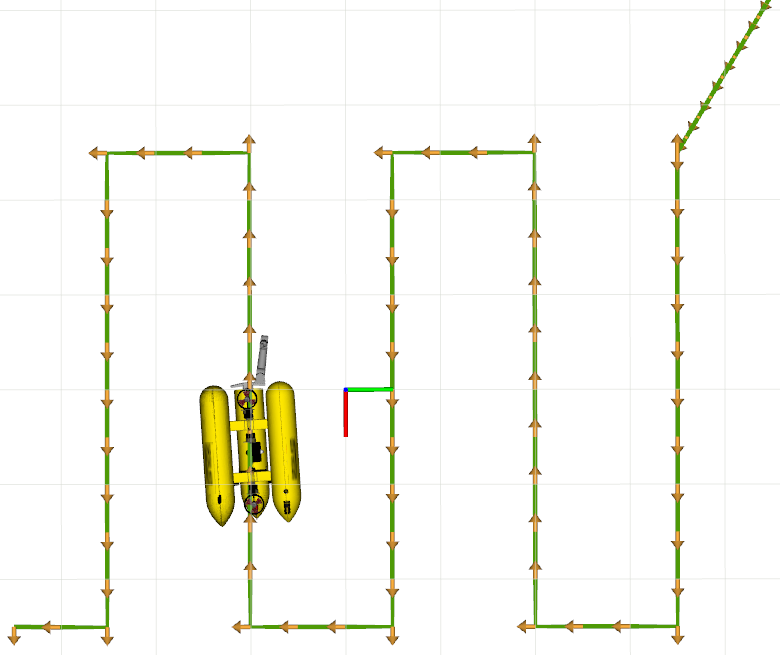
\includegraphics [width=\linewidth]{CameraReady/LaTeX/traj_rect.png}
\end{subfigure}
\hfill
\begin{subfigure}[b]{0.25\textwidth}
\centering
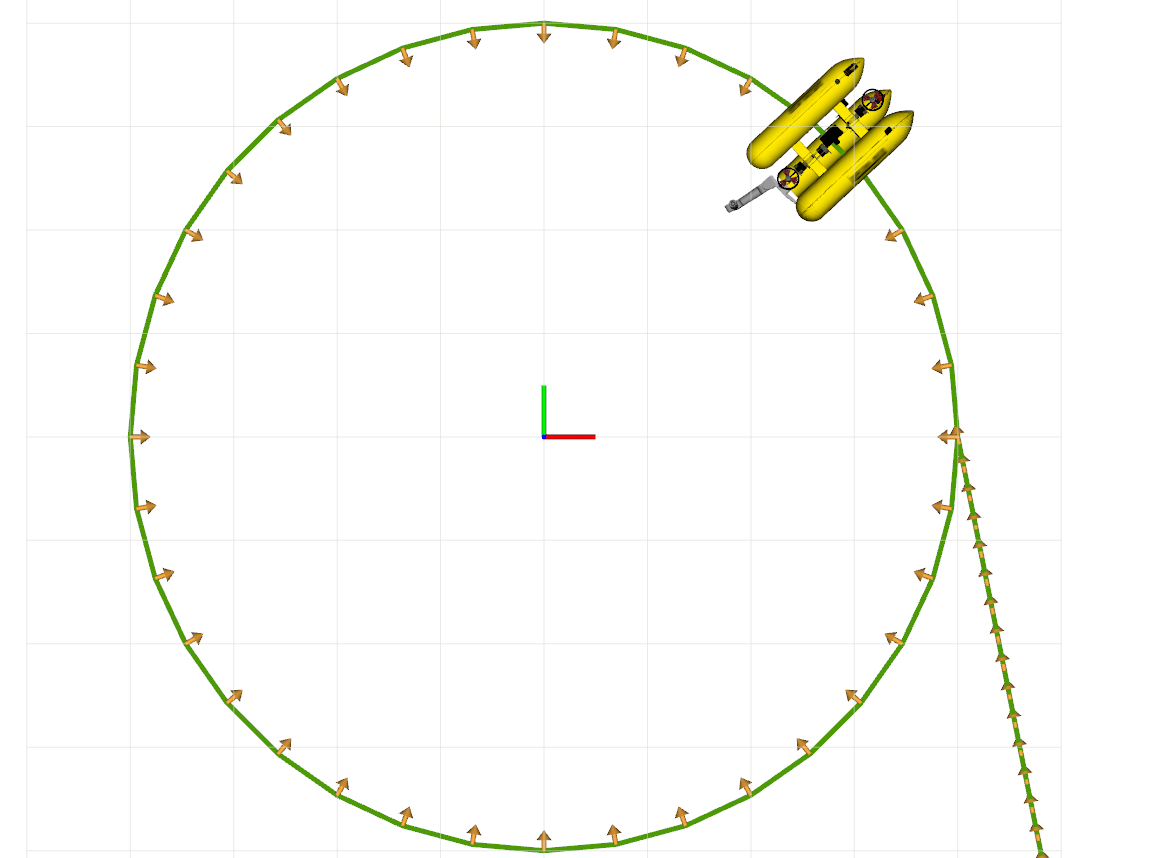
\includegraphics[trim={50 0 0 0},clip,width=0.9\linewidth]{CameraReady/LaTeX/traj_circ.png}
\end{subfigure}
\caption{Discovery and inspection trajectories generated by the RAG system.}
\label{fig:trajectories}

\end{figure}




\begin{figure}[t]
  \centering
  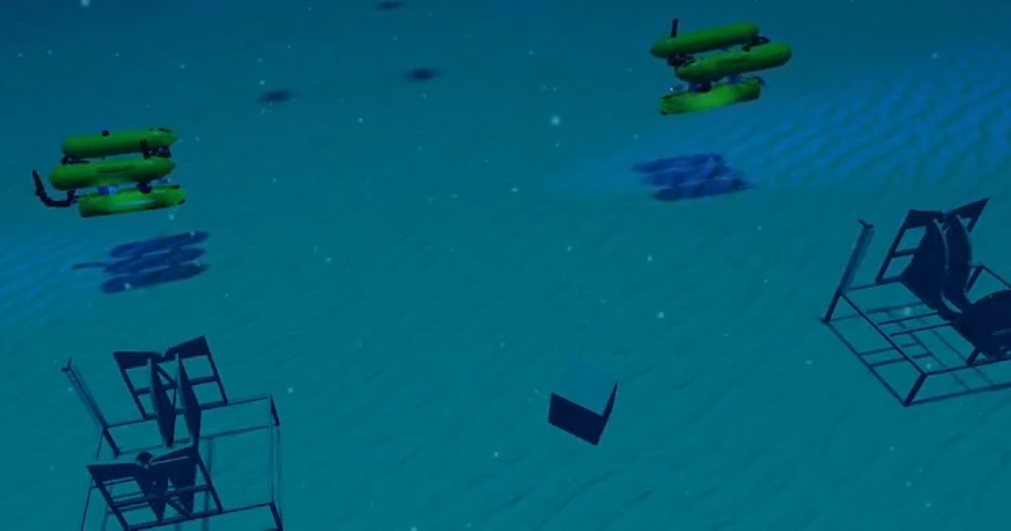
\includegraphics[width=0.95\linewidth]{CameraReady/LaTeX/two_auvs_comm}
 \caption{The two AUV using visual-light communication to share knowledge.}
  \label{fig:two_auv}
\end{figure}

\begin{figure*}[t]
  \centering
  
\includegraphics[width=0.95\linewidth]{CameraReady/LaTeX/architecture.png}
  \caption{Full and shared autonomy use-case schema. }
  \label{fig:use_case_system_architecture}
\end{figure*}



\section{Results}












\begin{figure*}
        \centering %
        \begin{subfigure}{0.33\textwidth}
          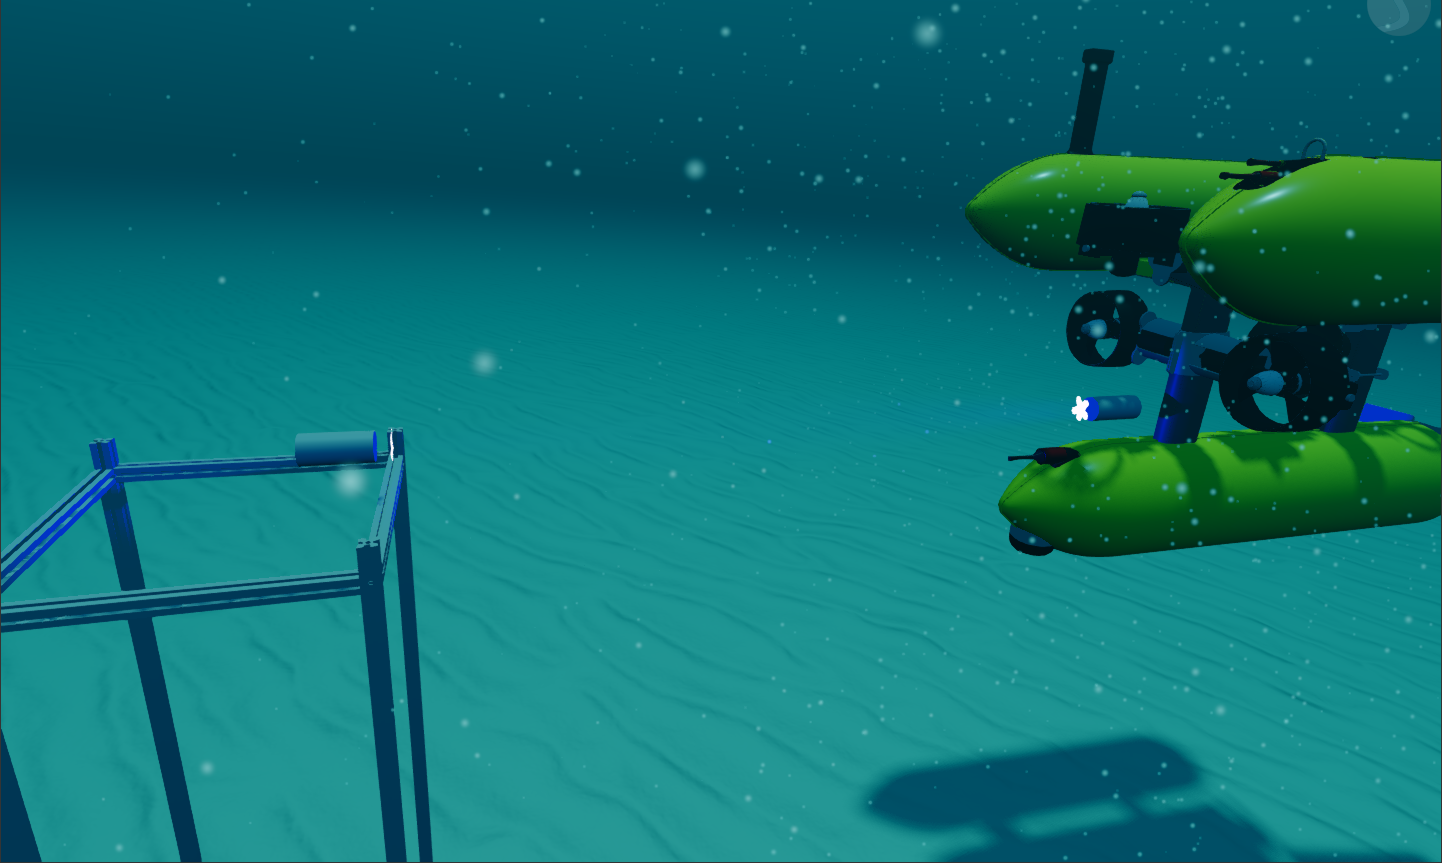
\includegraphics[width=\linewidth,height=4cm]{CameraReady/LaTeX/clear_g1000.png}
          \caption{VLC}
          \label{fig:vlc_clean}
        \end{subfigure}\hfil %
        \begin{subfigure}{0.33\textwidth}
          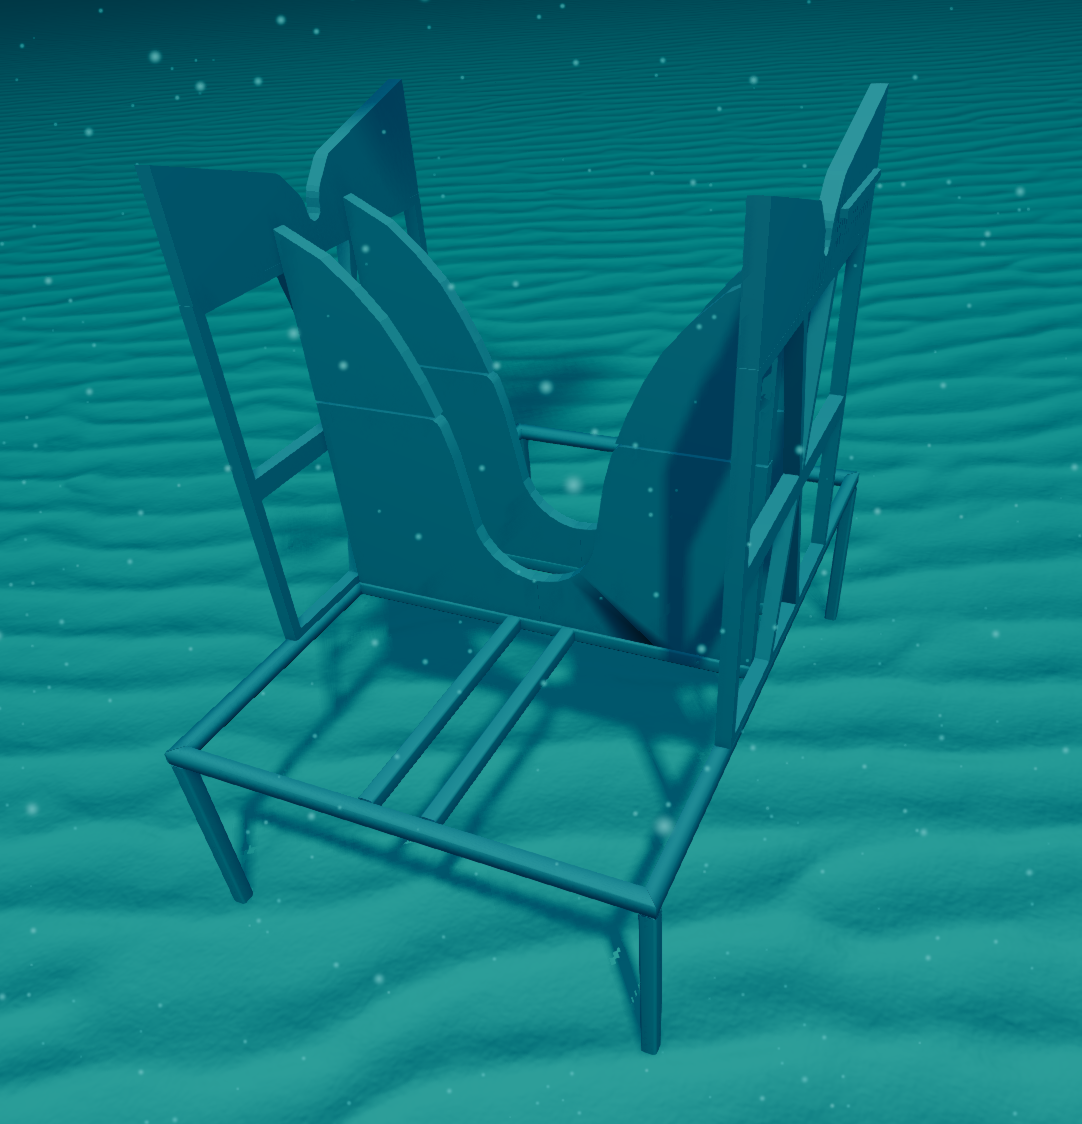
\includegraphics[width=\linewidth,height=4cm]{CameraReady/LaTeX/ds.png}
          \caption{Docking station}
          \label{fig:ds}
        \end{subfigure}\hfil %
        \begin{subfigure}{0.33\textwidth}
          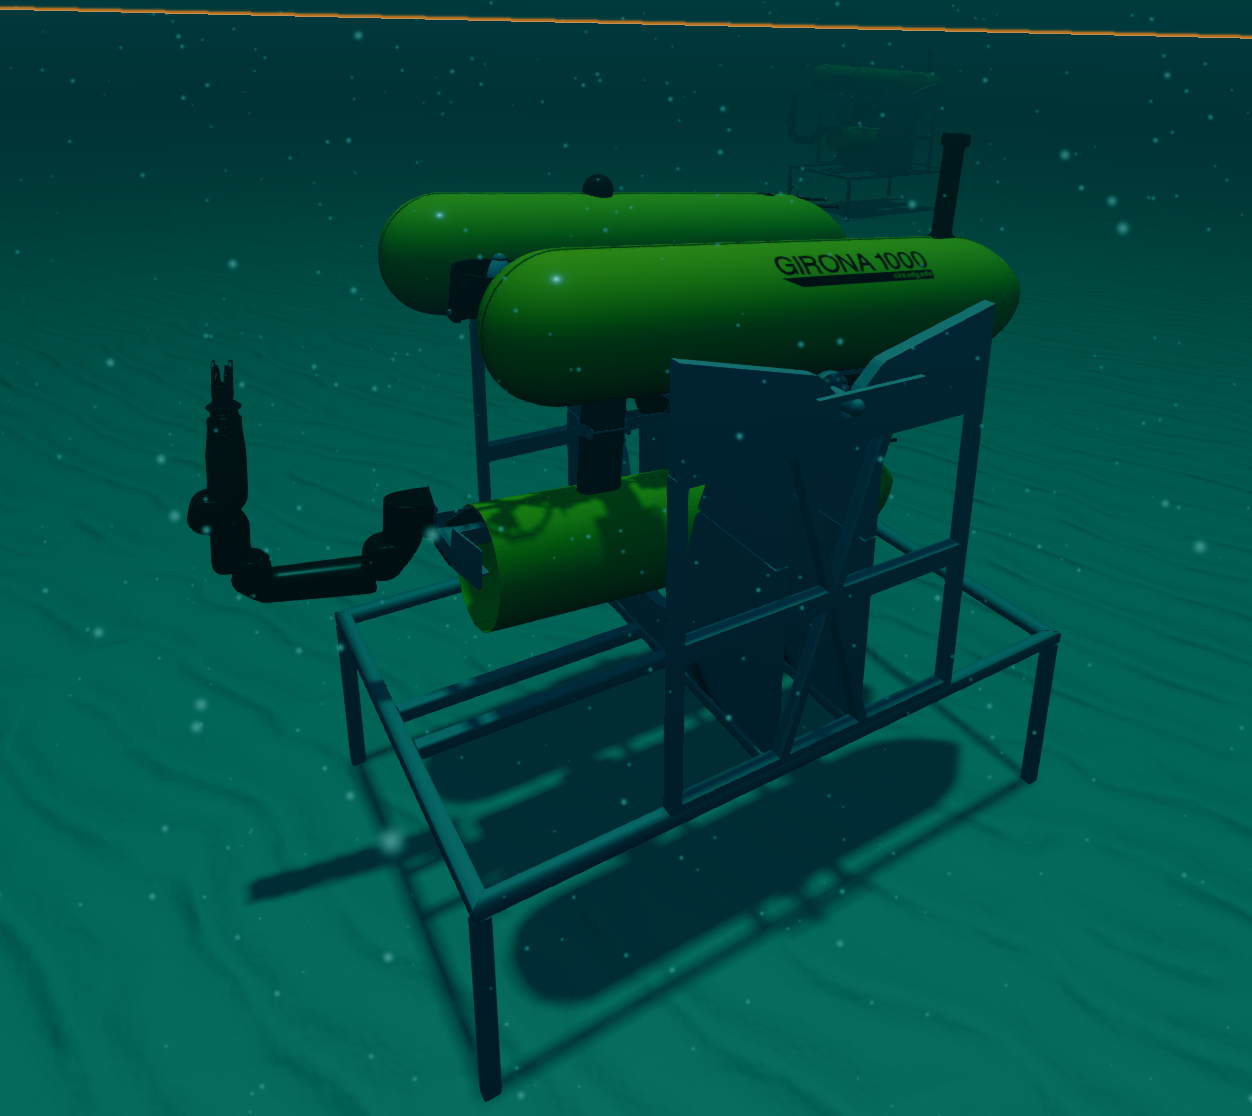
\includegraphics[width=\linewidth,height=4cm]{CameraReady/LaTeX/AUVInDS.png}
          \caption{AUV in Docking station}
          \label{fig:auv_in_ds}
        \end{subfigure}\hfil %
         \vspace{0.5cm}
          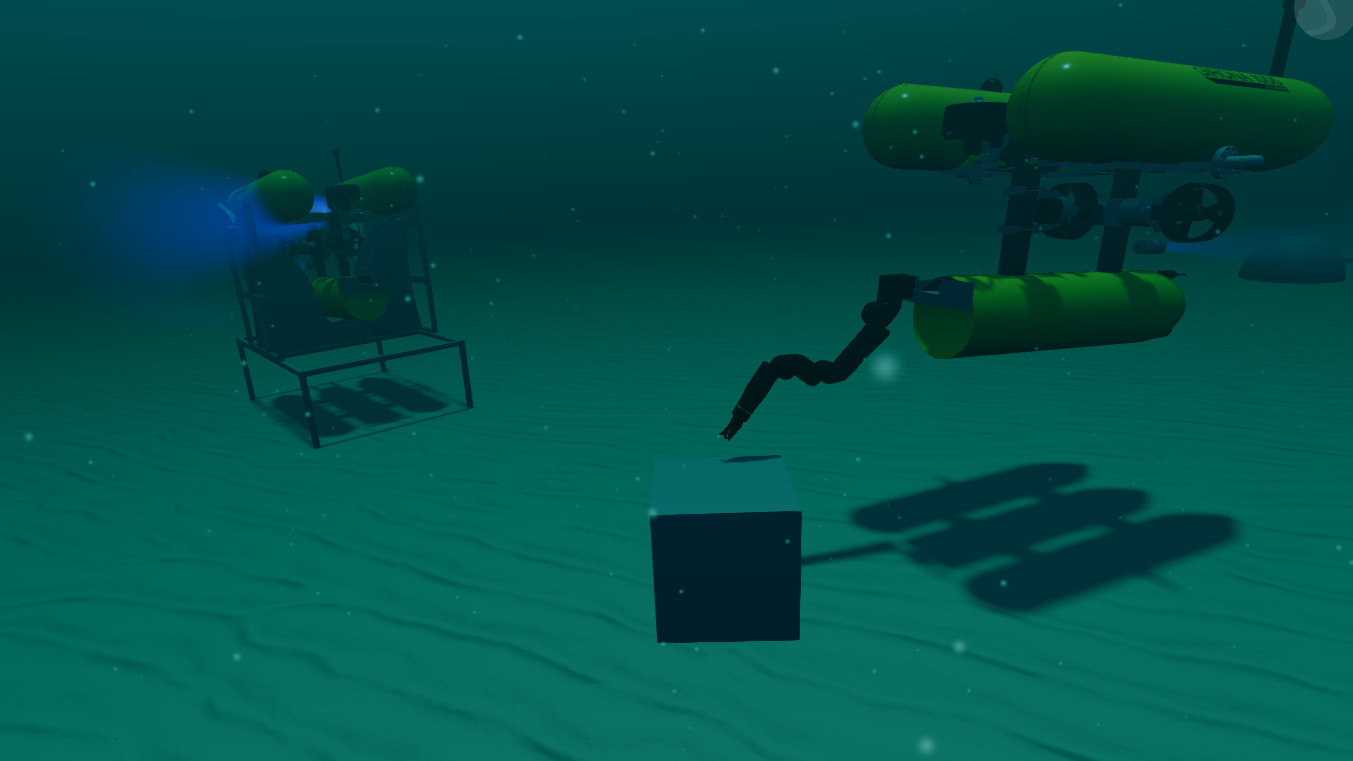
\includegraphics[width=0.45\linewidth]{CameraReady/LaTeX/touching.jpeg}
    \caption{Operational environments for the AUV: (a) VLC mounted on the docking station for communication, (b) docking station setup, and (c) the AUV docked for recharging or maintenance. Bottom: AUV \textit{Beta} interacting with an object, while \textit{Alpha} is recharging at the docking station.}
    \label{fig:ds_fig}
\end{figure*}










\begin{table*}[h]
\centering
\normalsize
\begin{tabular}{|l|c|c|}
\hline
\textbf{Method} & \textbf{Mission Validation Success Rate} & \textbf{BT Completeness} \\
\hline
LLM \& Runtime State + Knowledge Graph + Taxonomy & 100\% & 100\% \\
LLM \& Runtime State  + Knowledge Graph & 85\% & 76\% \\
LLM \& Runtime State & 21\% & 15\% \\
\hline
\end{tabular}
\caption{Comparison of RAG system configurations in terms of mission validation success and Mission Completeness (BT creation per task). Results are based on 20 missions per configuration.}
\label{tab:rag_performance}
\end{table*}

The evaluation of the proposed RAG-based system focused on its effectiveness in mission validation and BT planning within a simulated multi-AUV operational scenario. A demonstration video showcasing the use case has been made available online\footnote{The video is available here: \url{https://michele1996.github.io/rag_full_shared_autonomy.github.io/}}
To assess the contribution of each system component, we conducted an ablation study using the following configurations, each of them having access to the runtime state information (robot state and perceived environment):

\begin{itemize}
    \item \textbf{LLM \& Runtime State + Knowledge Graph + Taxonomy:} Full integration of structured domain knowledge and semantic task constraints.
    \item \textbf{LLM \& Runtime State + Knowledge Graph:} Language model reasoning grounded in factual knowledge without predefined semantic structuring.
    \item \textbf{LLM \& Runtime State:} Pure language-based generation with no semantic knowledge integration.
\end{itemize}

Each configuration was evaluated on 20 distinct missions to measure its mission validation success rate and behavior tree (BT) completeness (i.e., whether a valid BT was created for each task). 
No external baselines were used, as this work introduces a novel architecture that is able to perform tasks not achievable by other works in the state of the art. As such, there are no directly comparable prior systems. Instead, the ablation study serves to isolate and quantify the impact of each knowledge integration component.
The performance metrics for each configuration are summarized in Table~\ref{tab:rag_performance}.

\subsection{Mission execution} 
The scenario starts with the mission for robot Alpha sent by the user via a simulated Wi-Fi antenna.
Prior to execution, the AUV's mission was validated by its respective RAG system, which leveraged the knowledge graph to verify that the robot possessed the necessary capabilities to accomplish its assigned tasks. Upon validation, Alpha's LLM, featuring the Semantic Knowledge and Runtime State, reasoned that the best approach would be to execute a lawnmower-style survey of the area and created the corresponding behavior tree. Followed by a second behavior tree for the reporting phase, where the AUV approached the human operator to relay performance feedback. After completing the survey, Alpha navigated to the docking station to align its VLC system for data exchange.

To stimulate collaborative behavior, we intentionally configured Alpha with a low battery level and introduced partial errors in its object segmentation module. As a result, when an object was incorrectly segmented and Alpha lacked sufficient power to continue, Beta was deployed by the human from its docking station. Its first mission is to communicate with Alpha and receive the information collected and the human feedback. In this case, Alpha shares a task with Beta: to inspect an object that was previously misclassified. Beta’s RAG system validates the initial part of the mission, and both AUVs are then instructed by their respective RAG systems to move to precise positions. This positioning enables Alpha to transfer its data to Beta via VLC, as illustrated in Figure \ref{fig:two_auv}. Once the data transfer was completed, Alpha was instructed to return to the docking station to conserve and restore power. Subsequently, Beta's RAG validated the second part of the mission and instructed it to proceed with the inspection and circumnavigation of the misidentified object, performing a refined segmentation to correct the error.








\subsection{Mission Validation Accuracy}
One of the most consistent and impactful findings was the reliability of the full RAG configuration in mission validation. The system was able to correctly assess whether a task was feasible for a given AUV, never assigning actions that exceeded vehicle capabilities. This outcome can be directly attributed to the incorporation of the knowledge graph, which provided detailed specifications of vehicle parameters such as sensor ranges, manipulation capabilities, battery endurance, and depth limits. The predefined taxonomy further enhanced this validation process by enforcing semantic alignment between tasks and AUV roles, preventing mismatches like assigning manipulation tasks to non-manipulator vehicles.

By contrast, the LLM-only configuration exhibited frequent failures in validation. Lacking awareness of operational constraints, the LLM often overestimated AUV capabilities or hallucinated nonexistent ones. For instance, it occasionally assigned ``object retrieval'' missions to vehicles without manipulators or planned high-depth surveys for shallow-water units. These errors underline the limitations of relying solely on language priors without factual or semantic grounding.

The LLM+KG configuration partially mitigated these failures by anchoring generation in accurate vehicle data. However, without the taxonomy, the system sometimes misapplied tasks to objects in ways that were logically plausible in general terms but semantically invalid according to the operational context. For example, the system might assign an ``inspect'' task to a cylindrical object that, per the predefined taxonomy, is not an object type meant to be inspected, whereas a cube might be considered a valid inspection target. These object-task relationships are defined explicitly in the taxonomy, and without it, the LLM lacked a clear mapping between object types and valid actions. This resulted in plausible-sounding but operationally inappropriate plans. 

\subsection{Planning via Behavior Trees}
In addition to validating tasks, the system was evaluated on its ability to produce complete and coherent Behavior Trees (BTs) for each mission. The fully integrated RAG system demonstrated high performance in this area, generating well-structured BTs that included all required subtasks and actions, correctly sequenced. For example, mission plans involving underwater inspection included the full sequence of ``survey'', ``navigate to target'', ``inspect target'', ``doc'' and ``undock'' with appropriate condition checks embedded at each step.

When the taxonomy was removed, the BTs produced (LLM+KG configuration) were more error-prone. Incomplete or redundant steps became more common, particularly in complex multi-phase tasks such as object interaction or area mapping. The taxonomy served as a blueprint for assembling BTs, providing reusable action templates, and ensuring structural consistency across similar tasks.

The LLM-only setup produced the least reliable BTs. Many were missing critical actions or contained illogical transitions (e.g., attempting to verify a condition after executing the dependent action). In several cases, the BTs violated AUV constraints entirely, planning for unsupported behaviors or incompatible task sequences. These failures further reinforce the need for external grounding in both factual and semantic dimensions.

Overall, the experimental results demonstrated a clear hierarchy of performance across the three configurations:

    The \textbf{full RAG system} achieved high reliability in both mission validation and plan generation, consistently producing feasible, executable tasks and coherent BTs.

    The \textbf{LLM+KG system} performed reasonably well in feasibility checks but struggled with structured planning due to the absence of semantic task templates.

    The \textbf{LLM-only system} exhibited frequent errors in both validation and planning, with high rates of hallucination and logical inconsistencies.

These findings underscore the necessity of structured, domain-specific grounding—through both factual knowledge graphs and semantic taxonomies—for robust decision-making in autonomous mission planning.

